\documentclass[../main]{subfiles}
\begin{document}
\setcounter{secnumdepth}{3}
    \chapter{実験}
    \section{実験の手順}
        提案した通路認識の手法を2つのフェーズに分けて検証する.
        1つ目のフェーズでは事前に実験環境で取得した画像データを用いて通路の認識ができるか検証する.
        また,2つ目のフェーズでは機体に搭載したカメラからリアルタイムに取得する画像データを用いて通路認識を行い,
        トポロジカルマップとシナリオによるナビゲーションに適用し,先行研究のLiDARを用いた手法と比較して有効性を検証する.
        実験環境は\fref{figure::3floor_map}に示す千葉工業大学津田沼キャンパス2号館3階の廊下とした.
        \begin{figure}[H]
         \centering
         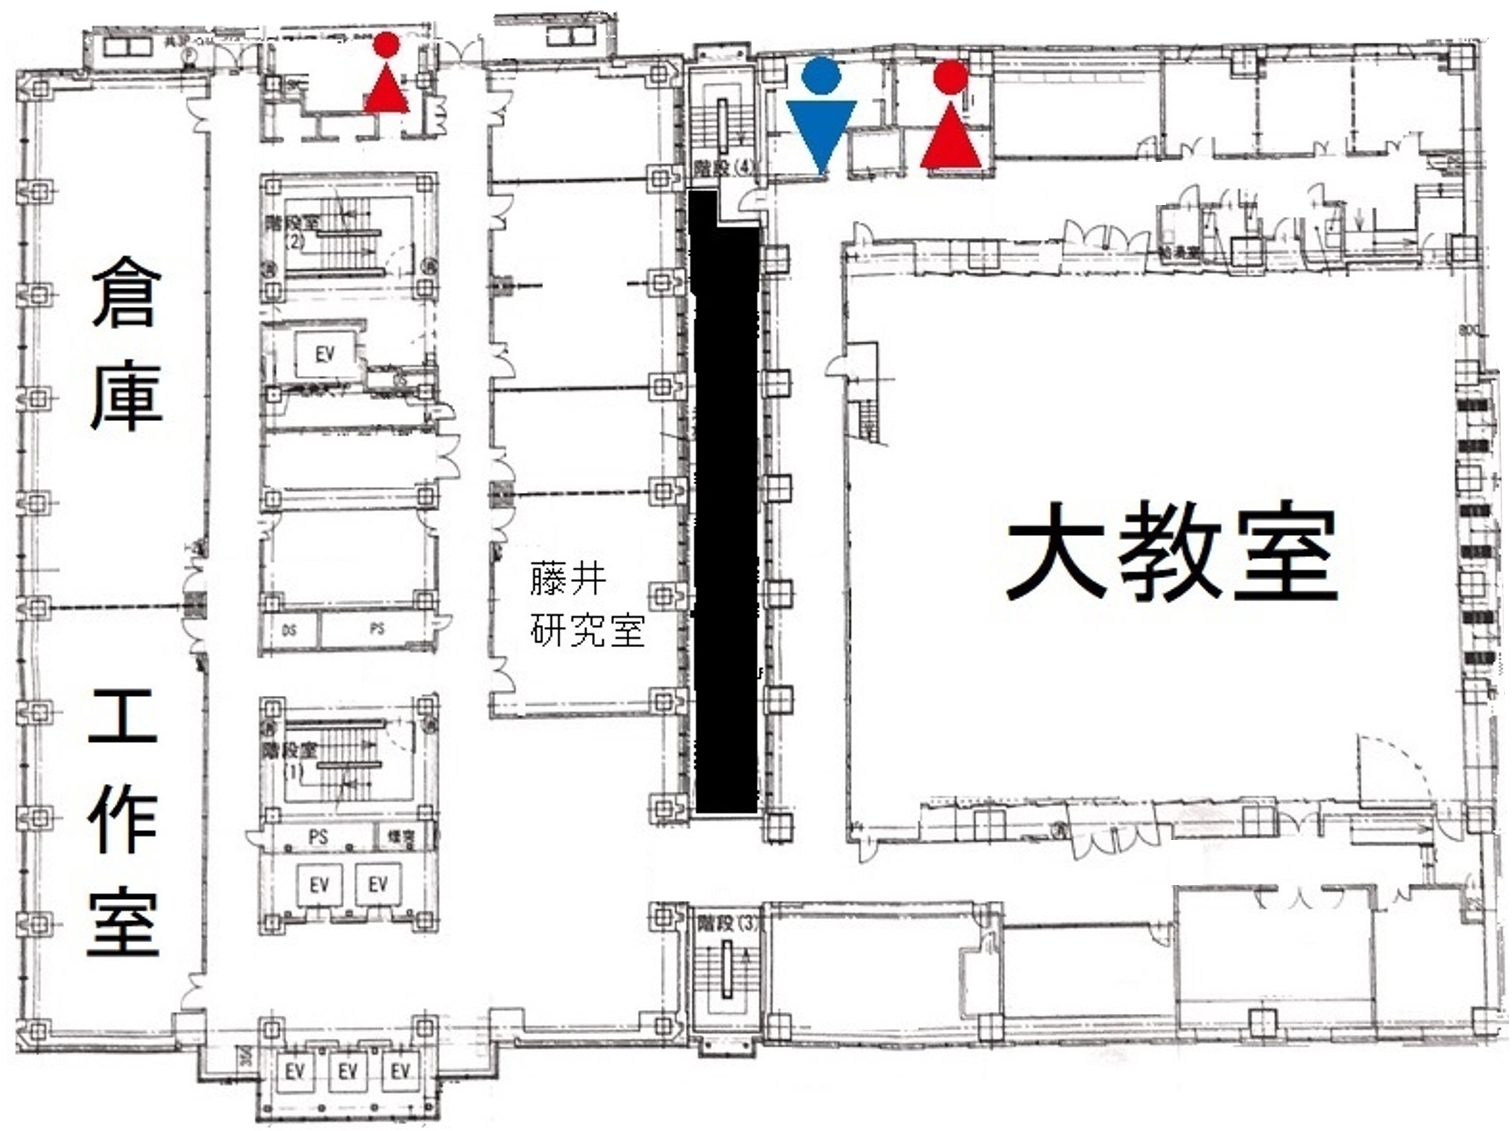
\includegraphics[width=15cm]{../images/MAP_Tsudanuma2-3.png}
         \caption{Experiment environment}
         \label{figure::3floor_map}
        \end{figure}

    \section{実験装置}
        実験には本研究室で開発をしているORNE-αを用いた.また,機体とその構成,使用したPCのスペックをそれぞれ
        \fref{figure::robot_image},\tref{table::robot_spec},\tref{table::pc_spec}に示す.
        

        \begin{figure}[H]
        \centering
        \includegraphics[width=7cm]{../images/robot_figure1.png}
        \caption{ORNE-α}
        \label{figure::robot_image}
        \end{figure}

        \begin{table}[H]
         \centering
         \caption{Specification of PC}
         \begin{tabular}{l|l} \hline
         \multicolumn{1}{c|}{CPU} & \multicolumn{1}{c}{Core i7-9750H(Intel)} \\ \hline
         \multicolumn{1}{c|}{RAM} & \multicolumn{1}{c}{16GB} \\ \hline
         \multicolumn{1}{c|}{GPU} & \multicolumn{1}{c}{RTX 2070 Max-Q} \\ \hline
         \end{tabular}
         \label{table::pc_spec}
        \end{table}

        \begin{table}[H]
            \centering
            \caption{Specification of ORNE-α}
            \begin{tabular}{l|l}\hline
            \multicolumn{1}{c|}{item}                                                              & \multicolumn{1}{c}{ORNE-α}                              \\ \hline
            \multicolumn{1}{c|}{Depth{[}mm{]}}                                                     & \multicolumn{1}{c}{710} \\ \hline
            \multicolumn{1}{c|}{Wide{[}mm{]}}                                                      & \multicolumn{1}{c}{560}                                 \\ \hline
            \multicolumn{1}{c|}{Height{[}mm{]}}                                                    & \multicolumn{1}{c}{810}                                  \\ \hline
            \multicolumn{1}{c|}{Weight{[}kg{]}}                                                    & \multicolumn{1}{c}{20}                                   \\ \hline
            \multicolumn{1}{c|}{\begin{tabular}[c]{@{}c@{}}Wheel diameter\\ {[}mm{]}\end{tabular}} & \multicolumn{1}{c}{304}                                   \\ \hline
            \multicolumn{1}{c|}{2D LiDAR(front)}                                                   & \multicolumn{1}{c}{Hokuyo URM-40LC-EW}                   \\ \hline
            \multicolumn{1}{c|}{2D LiDAR(back)}                                                    &                                        \\ \hline
            \multicolumn{1}{c|}{IMU}                                                               & \multicolumn{1}{c}{Analog devices ADIS16465-2BMLZ}         \\ \hline
            \multicolumn{1}{c|}{Battery}                                                           & \multicolumn{1}{c}{LONG WP12-12 × 2}                      \\ \hline
            \multicolumn{1}{c|}{Motor}                                                             & \multicolumn{1}{c}{Oriental motor TF-M30-24-3500-G15L/R}  \\ \hline
            \end{tabular}
            \label{table::robog_spec}
            \end{table}

    \section{実験1 事前取得のデータを用いた通路認識の検証}
        \subsection{実験目的}
        実験1では,あらかじめ実験環境で取得していた画像データを用いて通路の認識ができるか検証する.
        \subsection{実験方法}
        実験環境で取得した\fref{figure::}に示すような画像をYOLOに入力し,出力されたバウンディングボックスの情報とクラスの属性情報をテキストファイルに保存する.
        次に,保存したテキストファイルを読み込み,通路のタイプを判定する.
        用意した画像12枚を上記の方法で1枚ずつ読み込み,そこに写っている通路の認識を行う.

        \subsection{結果}

        \subsection{考察}
    \section{実験2 ナビゲーション適用時の通路認識の検証}
        \subsection{実験目的}

        \subsection{実験方法}

        \subsection{結果}

        \subsection{考察}
\end{document}